\documentclass[../Main/Knit.tex]{subfiles}

\section{Introduction}

Following the accurate characterisation of the mouse transcriptome using long-read sequencing from a global (whole transcriptome approach, \cref{wholetranscriptome}) and targeted perspective (Chapter \cref{targetedmousetranscriptome}), this chapter aims to exploit these datasets to investigate the transcriptional changes in the mouse entorhinal cortex associated with tau pathology. 

There have been multiple studies recently that explore the transcriptional differences in transgenic mice harbouring different mutations associated with AD. However, all of these studies to date have been undertaken with short-read RNA-Seq - which, while it offers obvious advantage compared to microarrays in accurately quantifying gene expression, is severely limited in detecting and characterising transcripts (as discussed in detail in \cref{rnaseq_intro}).

While there have been significant advances to process long-read sequencing data for transcriptome annotations, methods to harness long-read data for differential analyses have been limited. Currently, all the new tools developed to process long-read sequencing data (such as Oxford Nanopore's recommended cDNA transcriptome tutorial \cite{ONTcdna_transcriptome}, \textit{FLAIR} \cite{Tang2020}) integrate old tools, which were initially designed to analyse short-read sequencing data, for differential gene and isoform analyses. Systematically assessed and benchmarked for detecting differential splicing and expression at isoform level in RNA-Seq studies, \textit{DESeq2}, \textit{DexSeq} and \textit{NOISeq} have been most widely used. 
  

\section{Methods}
\subsection{Differential expression analysis}
After trialling various ad-hoc methods, I chose to explore the transcriptomic changes between wildtype and transgenic mice with \textit{tappAS} (v1.0.0)\cite{DeLaFuente2020}, which was also developed by the same authors as \textit{SQANTI} (A.Conesa's group) and was recommended as an extension to the Iso-Seq pipeline for the functional annotations of isoforms. Accessible as a user-friendly Java application, \textit{tappAS} was chosen as the framework for differential expression analysis due to the flexibility to explore both genotype effects and progressive changes across age, and to optimise parameters as background scripts were fully accessible and clearly written.

\textit{tappAS} requires three inputs\cite{DeLaFuente2020}:
\begin{enumerate}
	\item An experimental design file, which allows comparisons to be made between two or more groups and/or over a time-course 
	\item A transcript-level functional annotation file, which is generated post \textit{SQANTI} using \textit{IsoAnnot} (another tool developed by A.Conesa's group, https://isoannot.tappas.org), as a "scaffold" for transcript-level annotations. For the purpose of this study, the annotation file would be the conglomerate, long-read defined transcriptome of all the samples merged. 
	\item A transcript level expression matrix, which can either be derived directly from the full-length long-read transcript counts, or from mapping and transcript quantification of short-reads to the long-read defined transcriptome using \textit{Kallisto}(v0.46.0). Raw transcript counts were tabulated per sample.  	 
\end{enumerate}

As a method comparison, the expression from both short- and long-read was used as quantification at the gene and transcript level, such that four differential analyses were performed using the whole and targeted transcriptome datasets (\cref{tab:dea_analyses_summary}). To explore the utility and power of long reads for transcriptome annotation, results from the differential gene analyses were also compared to that generated from I.Castanho's analyses \cite{Castanho2020}. 
%brief statement of isabel's analyses  

\begin{table}[h]
	\centering
	\begin{tabularx}{0.9\textwidth}{cccc}
		\toprule
		& Datasets                                         & Annotation                                                                                                          & Quantification   \\ \midrule
		1 & \multirow{2}{*}{Whole Transcriptome  (n = 12)}   & \multirow{4}{*}{\begin{tabular}[c]{@{}c@{}}Iso-Seq reads \\ processed using\\ bioinformatics pipeline\end{tabular}} & Iso-Seq FL reads \\
		2 &                                                  &                                                                                                                     & RNA-Seq reads    \\
		3 & \multirow{2}{*}{Targeted Transcriptome (n = 24)} &                                                                                                                     & Iso-Seq FL reads \\
		4 &                                                  &                                                                                                                     & RNA-Seq reads    \\ \bottomrule
	\end{tabularx}
	\caption[Differential Gene and Transcript Analyses for mouse transcriptome using whole and targeted Iso-Seq transcriptome datasets]%
	{Summary of the differential gene and transcript analyses for mouse transcriptome using whole and targeted Iso-Seq transcriptome datasets. Using the Iso-Seq defined transcriptome as the "scaffold" rather than mouse reference genome, the analyses primarily differed on the quantification input. FL - Full length.}
	\label{tab:dea_analyses_summary}
\end{table}

\boldheader{Count Normalisation}
% Discussion of expression 
%The choice to use quantification directly from long-reads or derived indirectly from short-reads is dependent on the read coverage. While there will be no assembly ambiguity in using the abundance counts from long-reads, the coverage from the whole transcriptome approach would be insufficient for meaningful quantitative analyses - as shown in the coverage with ERCC (see Figure \cref{fig:isoseq_whole_ercc}) with lowly-expressed transcripts not being detected. Conversely, this is unlikely to be a limiting factor for the targeted transcriptome approach given the saturation coverage of target genes with additional sequencing of off-target, highly-expressed genes (see Figure \cref{fig:isoseq_targeted_rate}). Consequently, the expression matrix input for the whole transcriptome analyses was derived from the short-read alignment, and from the long-read abundance for the targeted transcriptome analyses. 
Very lowly-expressed transcripts with a sum of expression value less than 1 CPM (counts per million\nomenclature{CPM}{Counts per million}) or a large variance (>100 Coefficient of Variation) across all the samples were removed to reduce noise. The raw transcript counts were then normalised using TMM normalisation \cite{Robinson2010} (Trimmed Mean of M-values\nomenclature{TMM}{Trimmed Mean of M-values}) to account for differences in library size (sequencing depth) and sample RNA library composition, which is particularly important when comparing samples from different genotypes. The difference in RNA composition is determined by calculating a "scaling factor" for each sample relative to a reference sample (sample with the least varying read counts), which is the weighted average of all the log2 ratio of transcript counts between the two samples (M-values). The weighted average does not consider log2 ratio of transcripts with significant differences ("biased" transcripts that are widely present in one sample and not the other, and vice versa) and of transcripts with highest or lowest expression, hence "trimmed mean", to avoid effect of outliers. Of note, TMM assumes that the majority of the transcripts are not differentially expressed. Gene abundance was deduced from the sum of normalised counts of associated isoforms, after removing transcripts with low or highly-varied expression values.     

\boldheader{Differential Gene and Isoform Expression Analysis}
To elucidate transcriptional changes for both genotype and longitudinal effects between two groups and over time, \textit{maSigPro} \cite{Conesa2006,Nueda2014,Conesa2017} was used for both differential gene and transcript expression analysis, implemented as part of \textit{tappAS}. Briefly, maSigPro performs a two-step regression strategy to first define a negative binomial general linearised models\cite{Nueda2014} for each gene or transcript, accounting for both genotype and age (Equation \cref{eq:dea_lm_masigpro}), and identify differentially expressed genes. A stepwise regression is then applied to identify the conditions for which the differentially expressed genes have statistically significant profiles.  

Adapting the model\cite{Conesa2006} to our scenario, let \textit{I} denote the genotype groups (wildtype - WT, transgenic - TG) and \textit{J} as the age (2, 4, 6, 8 months) for each particular group, and assuming that gene or transcript expression in measured in replicated samples (\textit{R}).  



\begin{myequation}[!h]
\begin{align}\label{eq:dea_lm_masigpro}
y_{ijr} =  \:&\beta_{0} + \beta_{1}D_{ijr} \nonumber
\\ &+ \delta_{0}T_{ijr} + \delta_{1}T_{ijr}D_{ijr}   \nonumber
\\ &+ \gamma_{0}T_{1ijr}^{2} + \gamma_{1}T_{ijr}^{2}D_{ijr} \nonumber
\\ &+ \lambda _{0}T_{ijr}^{3} + \lambda_{1}T_{ijr}^{3}D_{ijr} + \varepsilon_{ijr} \nonumber
\end{align}
where:
\begin{conditions*}
	y_{ijr} & normalised expression value for each gene or transcript in the situation \textit{ijr} (genotype group \textit{i} at age \textit{j} of replicate \textit{r}) \\
	D  &  dummy binary variable to distinguish between the genotype groups, whereby 0 refers to reference group (WT) and 1 refers to experimental group (TG) \\
	T  &  age at 2, 4, 6, 8 months described using a polynomial model with a degree of 3 \\
	\beta_{0}, \delta_{0}, \gamma_{0}, \lambda _{0} & regression coefficients for reference group (WT) relating to the age \\ 
	\beta_{1}, \delta_{1}, \gamma_{1}, \lambda _{1} & regression coefficients for the difference between the experimental group (TG) and reference group (WT) at each age  
\end{conditions*}
therefore, if:
\begin{conditions*}
	FDR(\beta_{1}) < 0.05 & significant expression difference between WT and TG at 2 months \\ 
	FDR(\delta_{0}) < 0.05 & significant expression difference in WT across 2 and 4 months \\
	FDR(\delta_{1}) < 0.05 & significant expression difference between WT and TG across 2 and 4 months \\
\end{conditions*}
\hspace*{10mm}...
\captionsetup{width=0.95\textwidth}
\caption[Linear regression model to determine differential gene and transcript expression]%
{\textbf{Linear regression model to determine differential gene and transcript expression}. The model, adapted from \textit{MaSigPro} and implemented as part of \textit{tappAS}, describes gene or transcript expression between two groups (WT - wildtype, TG - transgenic) at four different time points (age in months). FDR - False discovery rate}    
\end{myequation}

\begin{figure}[!htp]
	\centering
	\includegraphics[page=2,trim={0 5cm 0 4cm},scale = 0.45]{Tg4510_diff_figures.pdf}
	\captionsetup{width=0.95\textwidth}
	\caption[Different conditions modelled for exploring rTg4510 genotype across age]%
	{\textbf{Different conditions modelled for exploring rTg4510 genotype across age.} An example of six different models generated with \textit{maSigPro} using Equation \cref{eq:dea_lm_masigpro} for 2 experimental groups (WT - Wildtype/Control, TG - Transgenic/Case) across two time points/age (T1, T2). The regression coefficients from Equation \cref{eq:dea_lm_masigpro} - $\beta_{1}$, $\delta_{0}$, $\delta_{1}$ - refer to the different variables modelled, the significance of which can be used to infer whether there is a genotype, age or interaction effect. The significance is symbolised by the tick and cross, which refers to adjusted P-value (FDR) < 0.05 and > 0.05 respectively. A significance of  $\beta_{1}$ denotes to a statistically significant difference between WT and TG at T1 (Genotype effect),$\delta_{0}$ to a difference in WT over time (Age effect), and $\delta_{1}$ to a difference between WT and TG across age (Interaction effect). \\\\
	\textit{maSigPro} labels the coefficients in the results table as "CaseVsControl", "Time", "TimexCase" for $\beta_{1}$, $\delta_{0}$, $\delta_{1}$. In the case where there is more time points/ages (as experimented in the Targeted Transcriptome datasets), the significance for the additional regression coefficients relating to the additional time variables are reported (Time2, Time2xCase, Time3, Time3xCase)}   
	\label{fig:dea_model}
\end{figure}

A gene or transcript with different profiles between WT and TG mice would have a different corresponding regression model with a statistically significant coefficient (\cref{fig:dea_model}), and was considered differentially expressed if P-value adjusted for multiple testing, by controlling the false discovery rate (FDR\nomenclature{FDR}{False Discovery Rate}) with the Benjamin and Hochberg correction, was < 0.05 and R\textsuperscript{2} > 0.5. The R\textsuperscript{2} defines the proportion of deviance that was explained by the linear regression model ("goodness of fit"), whereby a recommended threshold of 0.5 was used to identify differentially expressed genes with meaningful biological implications \cite{Conesa2006}.

Following the identification of statistically significant gene models (\cref{fig:dea_model}), the specific conditions (phenotype or age-associated changes) for which the genes show statistically significant profile changes (the significant variables) were identified by using an iterative backward stepwise approach \cite{Conesa2017}. The procedure therefore first started with all the variables imputed (different phenotype x age at different time points). At each iteration step, the P-value associated to each variable was determined and only the variables with a P-value < 0.05 were retained. 

\boldheader{Differential Isoform Usage}
\label{ch:diu_method}
In addition to assessing expression changes across conditions through differential isoform expression analysis, the relative expression, and as such the usage, of these isoforms can also change (see \cref{intro:dtu}). A gene is therefore identified as exhibiting differential isoform usage (DIU) if the fraction of the associated isoforms (Isoform Fraction) is significantly altered between conditions, which could result in switching of the major isoform. 

In accounting for biological replicates, the isoform fraction (IF) for each isoform was defined as:

\begin{myequation}[!h]
	\begin{align}
	IF_{cig} = \frac{\bar{E}_{cig}}{\sum_{i=1}^{n}\bar{E}_{cig}}
	\end{align}
	where:
	\begin{conditions*}
		\hspace{3mm}\conj{E}\textsubscript{cig} & mean normalised expression for isoform \textit{i} associated to gene \textit{g} under condition \textit{c}\\
		\hspace{3mm}n  & total number of isoforms associated with gene \textit{g}
	\end{conditions*}
	\captionsetup{width=0.95\textwidth}
	\caption[Calculation of isoform fraction for differential isoform usage analysis]%
	{\textbf{Calculation of isoform fraction for differential isoform usage analysis}. Equation is adopted from \textit{tappAS}}    
\end{myequation}
 

Despite abundant evidence of widespread isoform diversity \cite{Wang2008}, most protein-coding genes have been reported to typically express a few dominant isoforms \cite{Gonzalez-Porta2013, Ezkurdia2015}, while the remaining are very lowly expressed and unlikely to be main contributors to the proteome \cite{Gonzalez-Porta2013}.As such, minor isoforms were filtered to avoid finding genes associated with differential isoform usage due to "flat" behaviour of these minor isoforms \cite{DeLaFuente2020} (relatively small non-negligible expression changes of minor isoforms in the opposing direction of the predominant isoforms). \textit{tappAS} provides two strategies to filter lowly-expressed isoforms: an isoform is only retained if its proportion relative to other isoforms is greater than the pre-specified threshold (default: proportion $>$ 10\%) in at least one sample, or alternatively if its proportion relative to the major isoform is below a pre-specified threshold (default: FC = 2). A major isoform is defined as the isoform with the highest expression across all the conditions, with the remaining isoforms annotated as minor. 

Implemented as an additional filtering step after \textit{tappAS} and recommended in other bioinformatic tools\cite{Vitting-Seerup2017}, lowly expressed genes were also filtered as there would be less confidence in isoform fraction used for determining genes with significant differential isoform usage.  

\clearpage 
\section{Results}


\subsection{Transcriptome abundance hierarchal between samples}
\textbf{Annotated genes}
Average XX of annotated genes (XX out of XX; range: XX, sd: XX) with an average length of XX was identified. No difference in number of annotated genes or distribution of isoforms in annotated genes was identified between Tg4510 and J20 mouse. Average XX full splice match isoforms were identified with no difference between Tg4510 and J20 mouse [Table X for breakdown]

Different splicing events annotated by SUPPA2. Reported differences in terms of numbers between types of splicing events in WT vs TG in Tg4510 and J20?

XX of known transcripts were identified to have intron retention; XX of known transcripts were identified to be fusion genes. XX of know transcripts identified to have non-sense-mediated decay. 


\subsection{Change in endogeneous expression}
%Check whether overexpression of human MAPT result in any unwanted, compensatory effects on equivalent mouse genes,as expression levels of mouse APP and MAPT should be slightly reduced, thereby suggesting no evidence that human transgene expression increase expression of directly-related mouse genes.
Supporting findings from \cite{Castanho2020}, human-specific MAPT sequences were only detected in CCS and FL reads from TG mice, confirming stable insertion and activation of MAPT transgene in TG mice. 

\subsection{Differential Gene Expression Analysis}

\boldheader{Whole Transcriptome}
Using the Iso-Seq defined transcriptome as annotation independent of the expression source, we observed widespread transcriptional consequences from rTg4510 genotype with robust gene expression differences between WT and TG mice. Using the normalised RNA-Seq read count (n = 29 TG, n = 30 WT) for abundance, 1,290 differentially-expressed genes were identified, the majority (n = 796 genes, 61.7\%) of which were also identified when using the mouse reference genome instead as annotation. Strikingly, despite the lower sequencing coverage and smaller sample size (n = 6 TG, n = 6 WT) sequenced using the long-read platform, a significant number of differentially-expressed genes (n = 446 genes) were also identified when directly using the normalised full-length Iso-Seq read count. Classification of the differentially expressed genes by effects (depicted in \cref{fig:dea_model}) further identified the majority (n = 316 genes) to be associated with tau pathology and progressive with age (\cref{fig:dea_model_num}, \cref{fig:dea_model_genexp}).

\begin{figure}[!htp]
	\centering
	\includegraphics[page=4,trim={0 20cm 0 0},clip,scale = 0.55]{WholeDifferentialAnalysis.pdf}
	\captionsetup{width=0.95\textwidth}
	\caption[Differentially expressed genes classified by conditions]%
	{\textbf{Differentially expressed genes were identified across all the different conditions, with most genes exhibiting an interaction effect of rTg4510 genotype and age} Shown is a bar plot of the number of differentially expressed genes (n = 446) classified by the different conditions, as modelled in \cref{fig:dea_model}. The differentially expressed genes were identified from the whole transcriptome datasets (WT = 6, TG = 6, across age 2 and 8 months) using Iso-Seq read counts as abundance. WT - Wildtype, TG - Transgenic.}    
	\label{fig:dea_model_num}
\end{figure}

\begin{figure}[!htp]
	\centering
	\includegraphics[page=5,scale = 0.55]{WholeDifferentialAnalysis.pdf}
	\captionsetup{width=0.95\textwidth}
	\caption[Examples of gene expression differing across conditions]%
	{\textbf{Differential expressed genes exhibiting genotype, age and interaction effects} Shown are examples of differentially expressed genes classified under the different models, using the whole transcriptome dataset (WT = 6, TG = 6, across age 2 and 8 months) using Iso-Seq read counts as abundance: \textbf{a} \textit{Herc2} with a genotype effect, \textbf{b} \textit{Kcng1} with a genotype and age effect, \textbf{c} \textit{Clnc3} with an age effect, and \textbf{d} \textit{Cd34}, \textbf{e} \textit{Unc93b1}, \textbf{f} \textit{Csf1r} and \textbf{g} \textit{Gjb2} with an interaction effect. Dotted lines represent the mean paths across ages.}   
	\label{fig:dea_model_genexp}
\end{figure}


Of the differentially-expressed genes identified using Iso-Seq reads alone, the top ranked tau-associated differentially-expressed genes that was found to be progressive with age in our previous analyse\cite{Castanho2020} was also recapitulated: \textit{Gfap}, which encodes for glial fibrillary acidic protein (GFAP\nomenclature{GFAP}{Glial Fibrillary Acidic Protein}), a cytoskeletal protein that acts as a marker for astrocyte activation and proliferation - its increased expression was reported to correlate with increased neurofibrillary tangles density in Alzheimer's disease entorhinal cortex tissues \cite{Muramori1998}. Higher GFAP levels have also be documented in cerebrospinal fluid (CSF) in patients with AD compared to healthy control \cite{Ishiki2016}, and more recently, in plasma of cognitively intact older adults at risk of AD \cite{Chatterjee2021}. 


\begin{figure}[htp]
	\begin{center}
		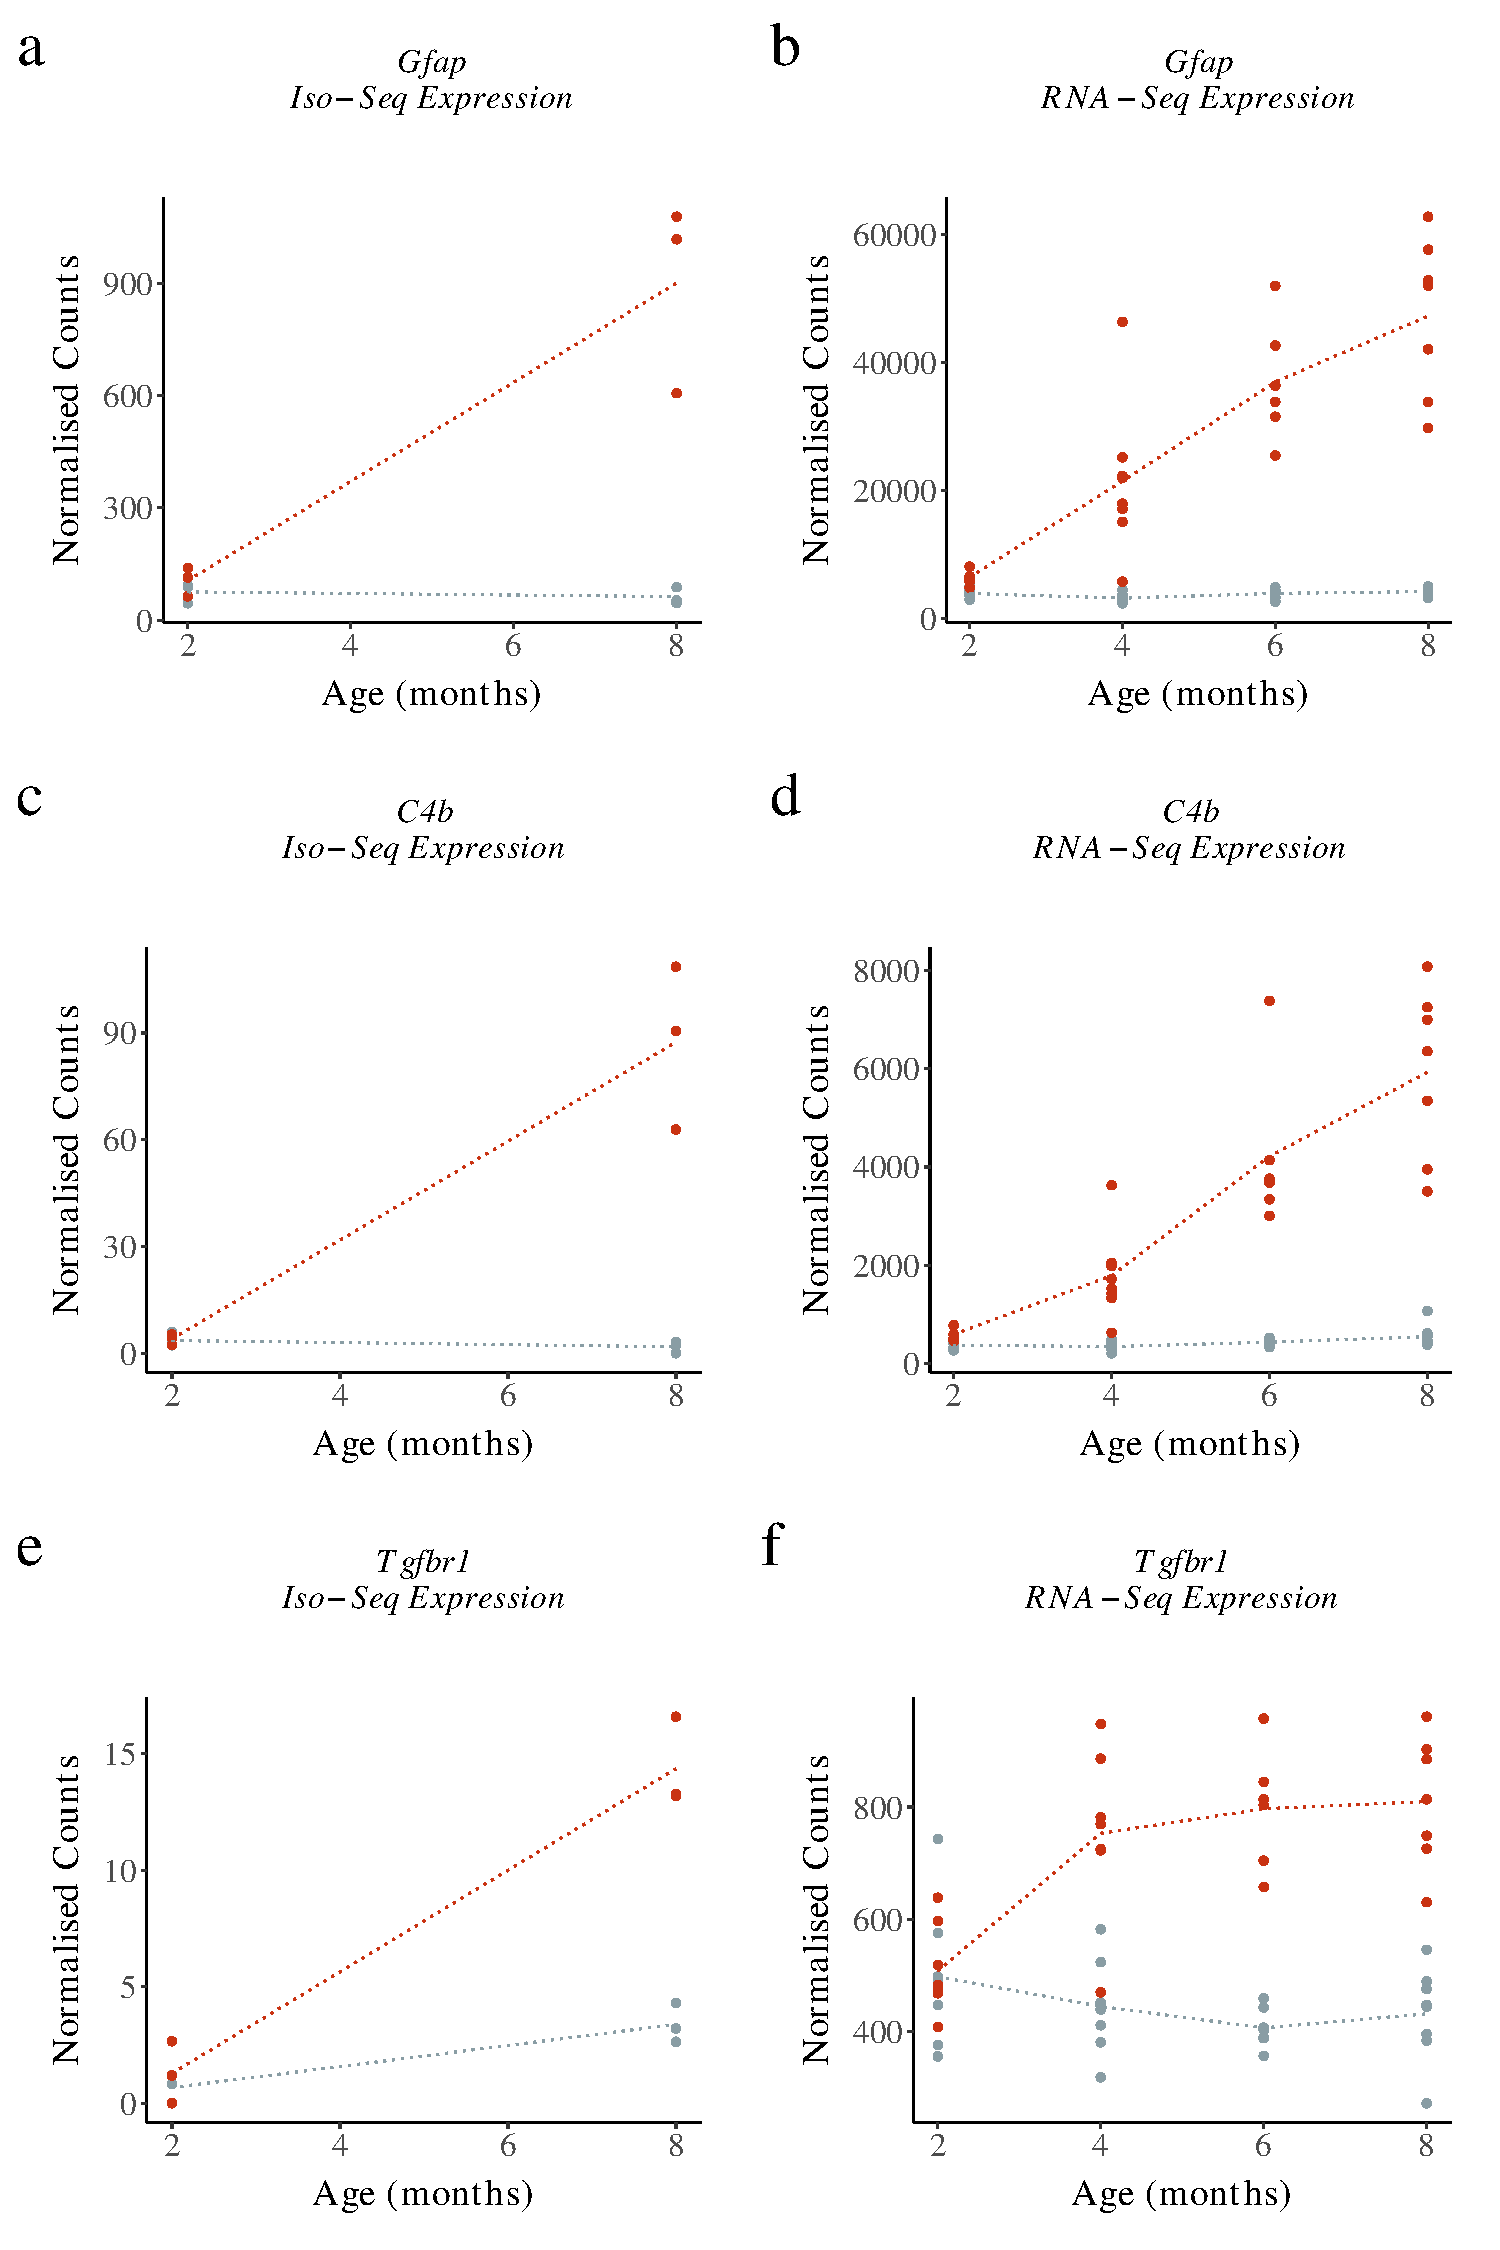
\includegraphics[page=1,scale = 0.55]{WholeDifferentialAnalysis.pdf}
	\end{center}
	\captionsetup{width=0.95\textwidth}
	\caption[Comparison of Known and Novel Isoforms from Iso-Seq Whole Transcriptome runs]%
	{\textbf{Novel isoforms were less expressed, longer and had more exons than known isoforms}: Shown is the \textbf{a)} Iso-Seq transcript expression, the \textbf{c)} transcript length, and the \textbf{e)} the number of exons of novel and known isoforms. The known and novel isoforms can be further subdivided and classified, with the \textbf{b)} Iso-Seq expression \textbf{d)} transcript length and \textbf{f)} number of exons for each category. According to SQANTI, known isoforms are subdivided into FSM and ISM, and novel isoforms are subdivided into NIC, NNC, and fusion. FSM – Full Splice Match, ISM – Incomplete Splice Match, NIC – Novel In Catalogue, NNC – Novel Not in Catalogue.}   
	\label{fig:whole_dea}
\end{figure}


%log2fc calculated by mean expression at 8 case/mean expression at 8 control
\begin{table}[]
	\centering
	\begin{tabularx}{0.96\textwidth}{cccccccc}
		\toprule
		\multirow{3}{*}{Gene} & \multirow{3}{*}{FDR} & \multirow{3}{*}{R\textsuperscript{2}} & \multirow{3}{*}{\begin{tabular}[c]{@{}c@{}}log2-fold \\ change \\ (8 months)\end{tabular}} & \multicolumn{4}{c}{Mean Gene Expression}                      \\ \cmidrule(l){5-8} 
		&                      &                    &                                                                                            & \multicolumn{2}{c}{Wildtype} & \multicolumn{2}{c}{Transgenic} \\ \cmidrule(l){5-8} 
		&                      &                    &                                                                                            & 2 months      & 8 months     & 2 months       & 8 months      \\ \midrule
		\textit{C4b}          & 3.9E-39              & 0.941              & 4.44                                                                                       & 3.57          & 1.79         & 4.03           & 87.4          \\
		\textit{Gfap}         & 8.88E-36             & 0.935              & 3.09                                                                                       & 75.6          & 62.3         & 106            & 900           \\
		\textit{Tgfbr1}       & 1.06E-20             & 0.880              & 3.48                                                                                       & 0.673         & 3.39         & 1.28           & 14.4          \\
		\textit{Slc14a1}      & 1.94E-16             & 0.872              & 2.92                                                                                       & 8.56          & 12.3         & 5.2            & 39.4          \\
		\textit{Unc93b1}      & 1.69E-15             & 0.853              & 1.5                                                                                        & 3.68          & 5.04         & 6.68           & 18.9          \\ \bottomrule
	\end{tabularx}
	\caption[Top-ranked differentially expressed genes associated with rTg4510]%
	{Tabulated are the top-ranked genes identified as differentially expressed in rTg4510 using \textit{maSigPro} with Iso-Seq defined transcriptome for annotation and Iso-Seq FL read count as expression. Gene expression is determined from the sum of normalised expression of associated transcripts. FDR - False Discovery Rate. }
	\label{tab:dea_wholemouse}
\end{table}


Other top-ranked differentially-expressed genes have been reported to be involved in AD development and pathology, notably \textit{C4b} - a member of the complement immune system, \textit{Slc14a1} encoding the urea transporter 1, \textit{Tgfbr1} encoding the TGF-\textbeta receptor protein and \textit{Unc93b1}, a transmemebrane protein required for toll (\cref{tab:dea_wholemouse}). Up-regulated expression of these genes have been observed previously in AD patients and other AD mouse models \cite{Zorzetto2016,Castillo2017,Wirz2013}. 

Using \textit{EnrichR}, differentially expressed genes (n = 466) were found to be highly enriched in lysosome (KEGG 2021 Human: odds ratio = 5.99, adjusted P = 4.41 x 10\textsuperscript{-6}) and in particularly the TGF-\textbeta pathway (WikiPathway 2021 Human: odds ratio = 58.98, adjusted P = 2.69 x 10\textsuperscript{-3} ). 

Correlating the significance (P-values) of genes identified as differentially expressed, the two analyses involving RNA-Seq reads as expression input were strongly correlated (RNA-Seq reads mapped to reference genome vs RNA-Seq reads mapped to Iso-Seq defined transcription: Spearman r = 0.534, P = 6.71 x 10\textsuperscript{-60}), which is a likely reflection of the relatively lower Iso-Seq sequencing depth. Conversely, no correlation was observed when compared to using Iso-Seq FL reads for expression (RNA-Seq reads mapped to reference genome vs Iso-Seq normalised expression: Spearman r = 0.132, P = 0.173; RNA-Seq reads mapped to Iso-Seq defined transcriptome vs Iso-Seq normalised expression: Spearman r = 0.12,  P = 0.173). Taken together, these results demonstrate the power of Iso-Seq at the whole transcriptome level for transcriptome annotation but the continued usage of RNA-Seq reads for accurate gene quantification, until a higher sequencing coverage can be achieved with Iso-Seq reads.

\subsection{Differential Isoform Expression Analysis}
One of the added advantages of long reads over short-reads is the power to accurately identify isoforms and to explore isoform expression changes across conditions and over time. Using \textit{MaSigPro} with Iso-Seq reads as both reference annotation and expression, we identified hundreds of differentially expressed isoforms (n = 583 isoforms), of which 37 (6.35\%) were associated with rTg4510 phenotype and interaction between phenotype and age (n = XX).

\subsection{Differential Isoform Usage Analysis}
Filtering of lowly-expressed isoforms using the two provided strategies (described in \cref{ch:diu_method}) and Iso-Seq reads for abundance yielded similar results with approximately ~400 genes characterised by differential isoform usage (DIU). However upon further examination, the majority of these genes were lowly expressed and the associated isoforms that were observed to undergo differential usage were only detected with 1-2 full-length long read count. We were therefore not confident in any of observed DIU changes detected with Iso-Seq abundance from the whole transcriptome sequencing due to low sequencing depth. Indeed, none of the DTU genes were significant after applying the gene expression threshold (described in \cref{ch:diu_method}).

In support of this conclusion, there was a low overlap of genes that were similarly identified with DIU when using RNA-Seq reads for abundance, independent of the filtering strategy used (n = 21 genes when filtering by proportion, n = 37 genes when filtering by fold change relative to major isoform). This was likely to be a reflection of the difference in sequencing depth between short- and long-reads, which resulted in a different pool of isoforms after filtering for lowly-expressed isoforms (a minor isoform was more likely to be filtered when using RNA-Seq reads as abundance rather than Iso-Seq reads, particularly if the overall gene expression was low, due to relatively greater expression difference). Interestingly, the was a lower consensus when comparing the number of DIU genes identified when using RNA-Seq reads as abundance, suggesting that the choice of filtering strategy becomes redundant when dealing with low sequencing depth.  

\begin{figure}[htp]
	\begin{center}
		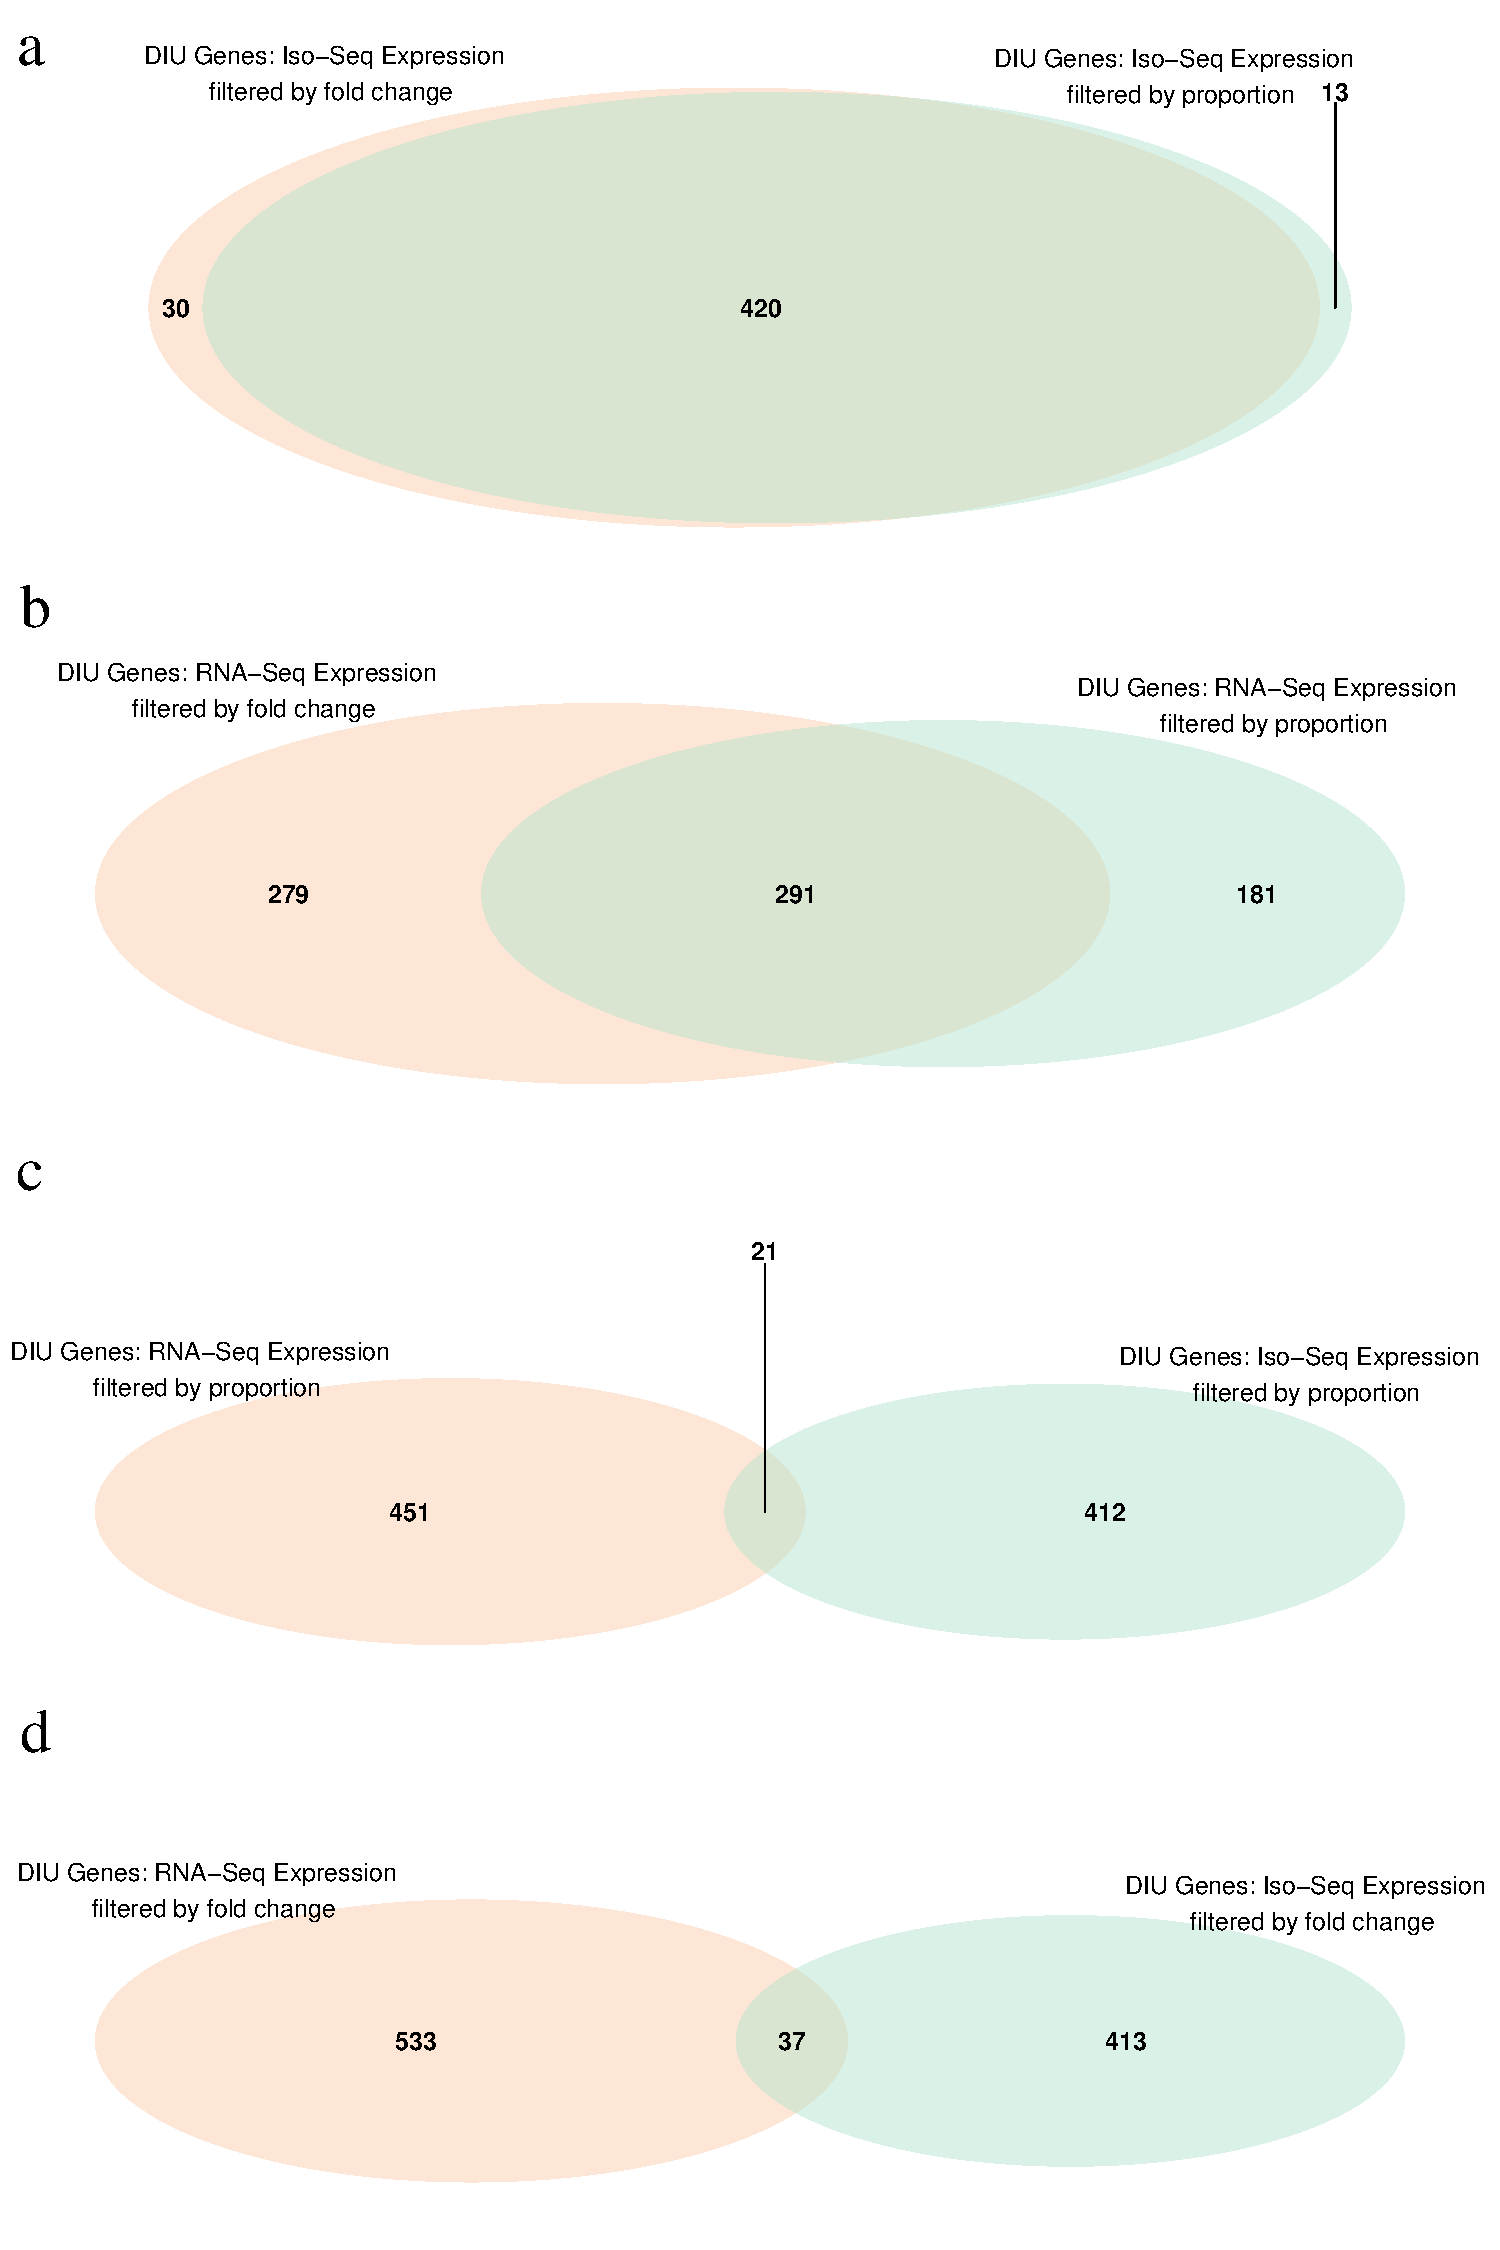
\includegraphics[page=1,scale = 0.55]{WholeDIUAnalysis.pdf}
	\end{center}
	\captionsetup{width=0.95\textwidth}
	\caption[Number of DIU genes identified from Whole Transcriptome mouse datasets]%
	{\textbf{Comparison of number of differentially expressed genes identified from Whole Transcriptome datasets after using RNA-Seq or Iso-Seq reads as abundance and various strategies to filter lowly-expressed isoforms}: Shown are venn diagrams that encapsulate the number of genes observed with significant differentially isoform usage, if \textbf{a)} Iso-Seq reads were used as abundance, and lowly expressed isoforms were pre-filtered either by relative proportion or fold change to major isoform, \textbf{b)} RNA-Seq reads were used as abundance, \textbf{c)} if relative proportion or \textbf{d)} relative fold change to major isoform, was chosen as strategy for filtering lowly-expressed isoforms }   
	\label{fig:whole_venn_diu_methods}
\end{figure}
